\chapter{Modellierung}
\label{chap:SEVN}
\minitoc

\section{Aufgabenstellung}
\label{sec:aufst}

%%%%%%%%%%%%%%%%%%%%%%%%%%%%%%%%%%%%%%%%%%%%%%%%%%%%%%%
%%%%%%%%%%%%%%%%%%%%%%%%%%%%%%%%%%%%%%%%%%%%%%%%%%%%%%%
%%%%%%%%%%%%%%%%%%%%%%%%%%%%%%%%%%%%%%%%%%%%%%%%%%%%%%%

Die Intention der Arbeit, ist im Ramen der Bereitstellung der Regelleistung
f\"ur erneuerbaren Energien durch den Einsatz der Verfahren und Techniken des
objektorientierten Entwurfs ein \matlab-Programm zur Simulation des variablen
Lastverhaltens von Kältelasten mit Kältespeichern im Energieversorgungsnetz zu
entwerfen. Anschliessend wird mit Hilfe des Programms das variable Verhalten der
K\"altespeicher im Enerergieversorgungsnetz simuliert und der Einfluss auf das
Energieversorgungsnetz untersucht.

Es sollen ausschlie\ss lich K\"alteanlagen modelliert werden, die in
Superm\"arkten zum Einsatz kommen. Das Ergebnis der Simulation soll der
Verbrauch einer variabel gef\"uhrten Supermarktkette auf der Basis der einzelnen
in den Superm\"arkten eingesetzten K\"alteanlagen sein.

Verbrauchswerte in einem Lastflussoptimierungsprogramm zu verwenden.

\subsection*{Explizite Anforderungen}

Folgende explizite Anforderungen sind an das Programm gestellt:

\begin{itemize}
	\item Der Entwurf des Programms erfolgt mit Hilfe der objektorientierter
	Verfahren und Techniken.
	\item Die Speicherung der f\"ur das Beschreiben der Modelle
	erforderlichen Parameter findet in einer Konfigurationsdatei statt.
	\item Der elektrische Energieverbrauch wird aufgrund der Modellparameter
	der Kältelasten sowie des gefahrenen Einsatzes der Kältelasten
	berechnet.
	\item Die Topologie des elektrischen Netzwerkes wird ber\"ucksichtigt.
	\item Die M\"oglichkeit einer eindeutigen Zuweisung der Verbrauchswerte
	f\"ur folgende Verursacher wird realisiert:
	\begin{itemize}
		\item Die berechneten Werte f\"ur jede K\"alteanlage werden
		einzeln gespeichert, wenn mehrere Anlagen simuliert werden.
		\item Die berechneten Werte f\"ur jede Supermarktkette werden
		einzeln gespeichert, wenn der Verbrauch mehrerer
		Supermarktketten simuliert wird.
	\end{itemize}
	\item Eine M\"oglichkeit zur graphischen Auswertung der Berechnung wird
	erstellt.
\end{itemize}


%%%%%%%%%%%%%%%%%%%%%%%%%%%%%%%%%%%%%%%%%%%%%%%%%%%%%%%%%%%%%%%%%%%%%%%%%%%%%%%%
%%%%%%%%%%%%%%%%%%%%%%%%%%%%%%%%%%%%%%%%%%%%%%%%%%%%%%%%%%%%%%%%%%%%%%%%%%%%%%%%

\section{Erstellung des OOP-Modells}

Der durchschnittliche Energieverbrauch der Kälteanlagen je Supermaktkette
kann aufgrund der technischen Ausführung unterschiedlich ausfallen. Der
Energieverbrauch entsteht an definierten Punkten im Netz. An den einzelnen
Knotenpunkten können mehrere Kältelasten angeschlossen sein.\\

In der \cref{fig:vkb} wird ein einfaches Energieversorgungsnetz mit vier Knoten
dargestellt. Am Knoten eins ist eine regenerative elektrische Energiequelle, in
diesem Fall ein Windpark, angeschlossen. Weitere konventionelle elektrische
Energiequellen befinden sich an den Knoten zwei und drei. Die passiven Lasten
befinden sich am Knoten zwei und vier. Der Kältespeicher ist am Knoten zwei
angeschlossen. Im Bild wird der Kältespeicher Supermarkt durch ein Geb\"aude
mit Einkaufswagen dargestellt. Die Knoten sind untereinander durch Leitungen
verbunden.

\begin{figure}[h]
	\begin{center}
	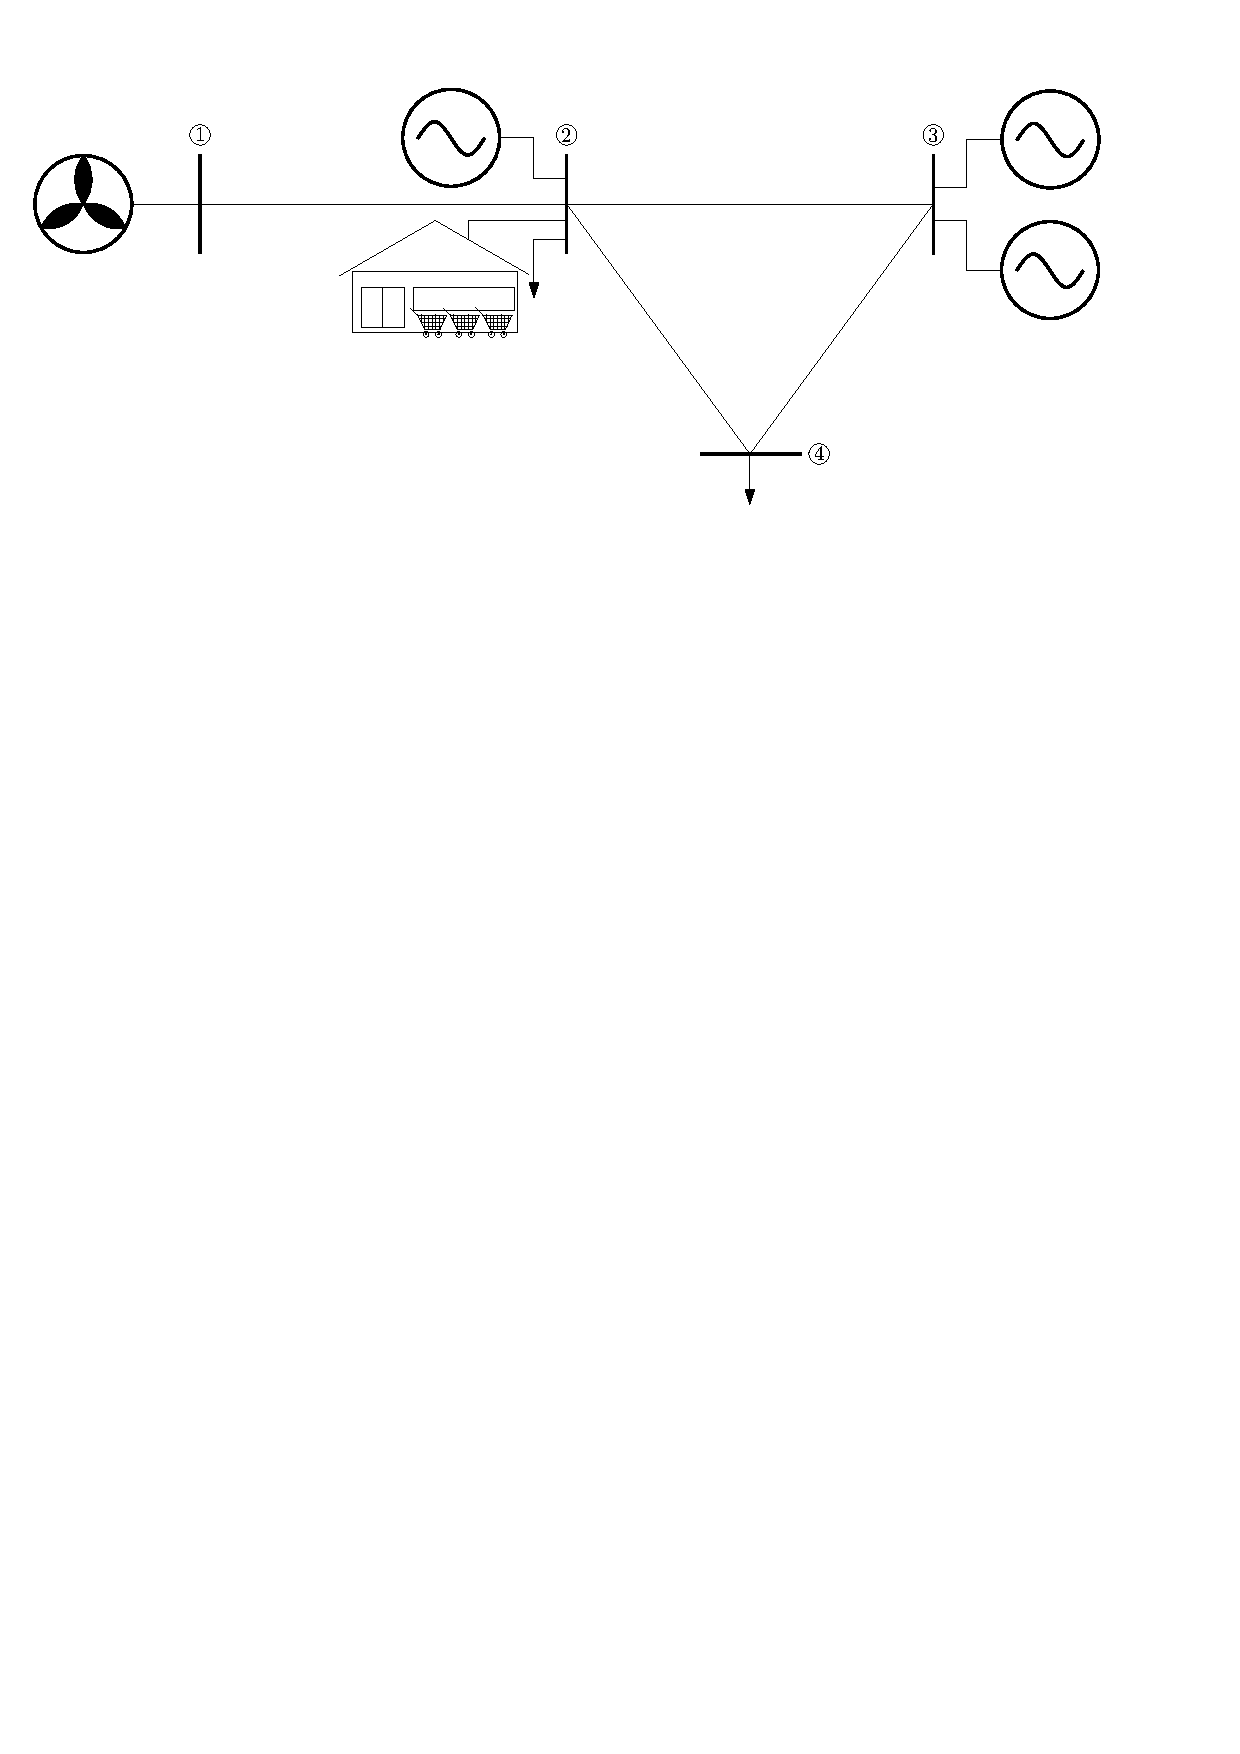
\includegraphics[scale=0.75]{images/SEVN/power_grid}
	\end{center}
\caption{Vier Knoten Beispiel}
\label{fig:vkb}
\end{figure}

\noindent In der Realität kann ein Energieversorgungsnetz durch die Variation
der Knotenzahl und die Vermaschung eine beliebig komplizierte Form aufweisen. \\

In Anbetracht der im \cref{sec:OOP} vorgestellten Verfahren erscheint der Ansatz
der OOP bei der Erstellung eines Programms zur Simulation einer K\"alteslast mit
K\"altespeicher im Energieversorgungsnetz auf der Basis des vorangegangenen
Beispiels (\cref{fig:vkb} auf der Seite \pageref{fig:vkb}) als sinnvoll. In der
\cref{fig:klassendiagramm} auf der Seite \pageref{fig:klassendiagramm} wird in
Form eines Klassendiagramms das fertige Klassen-Modell dargestellt und die
Abh\"angigkeit unter Klassen visualisiert.

\begin{figure}[h!]
	\begin{center}
	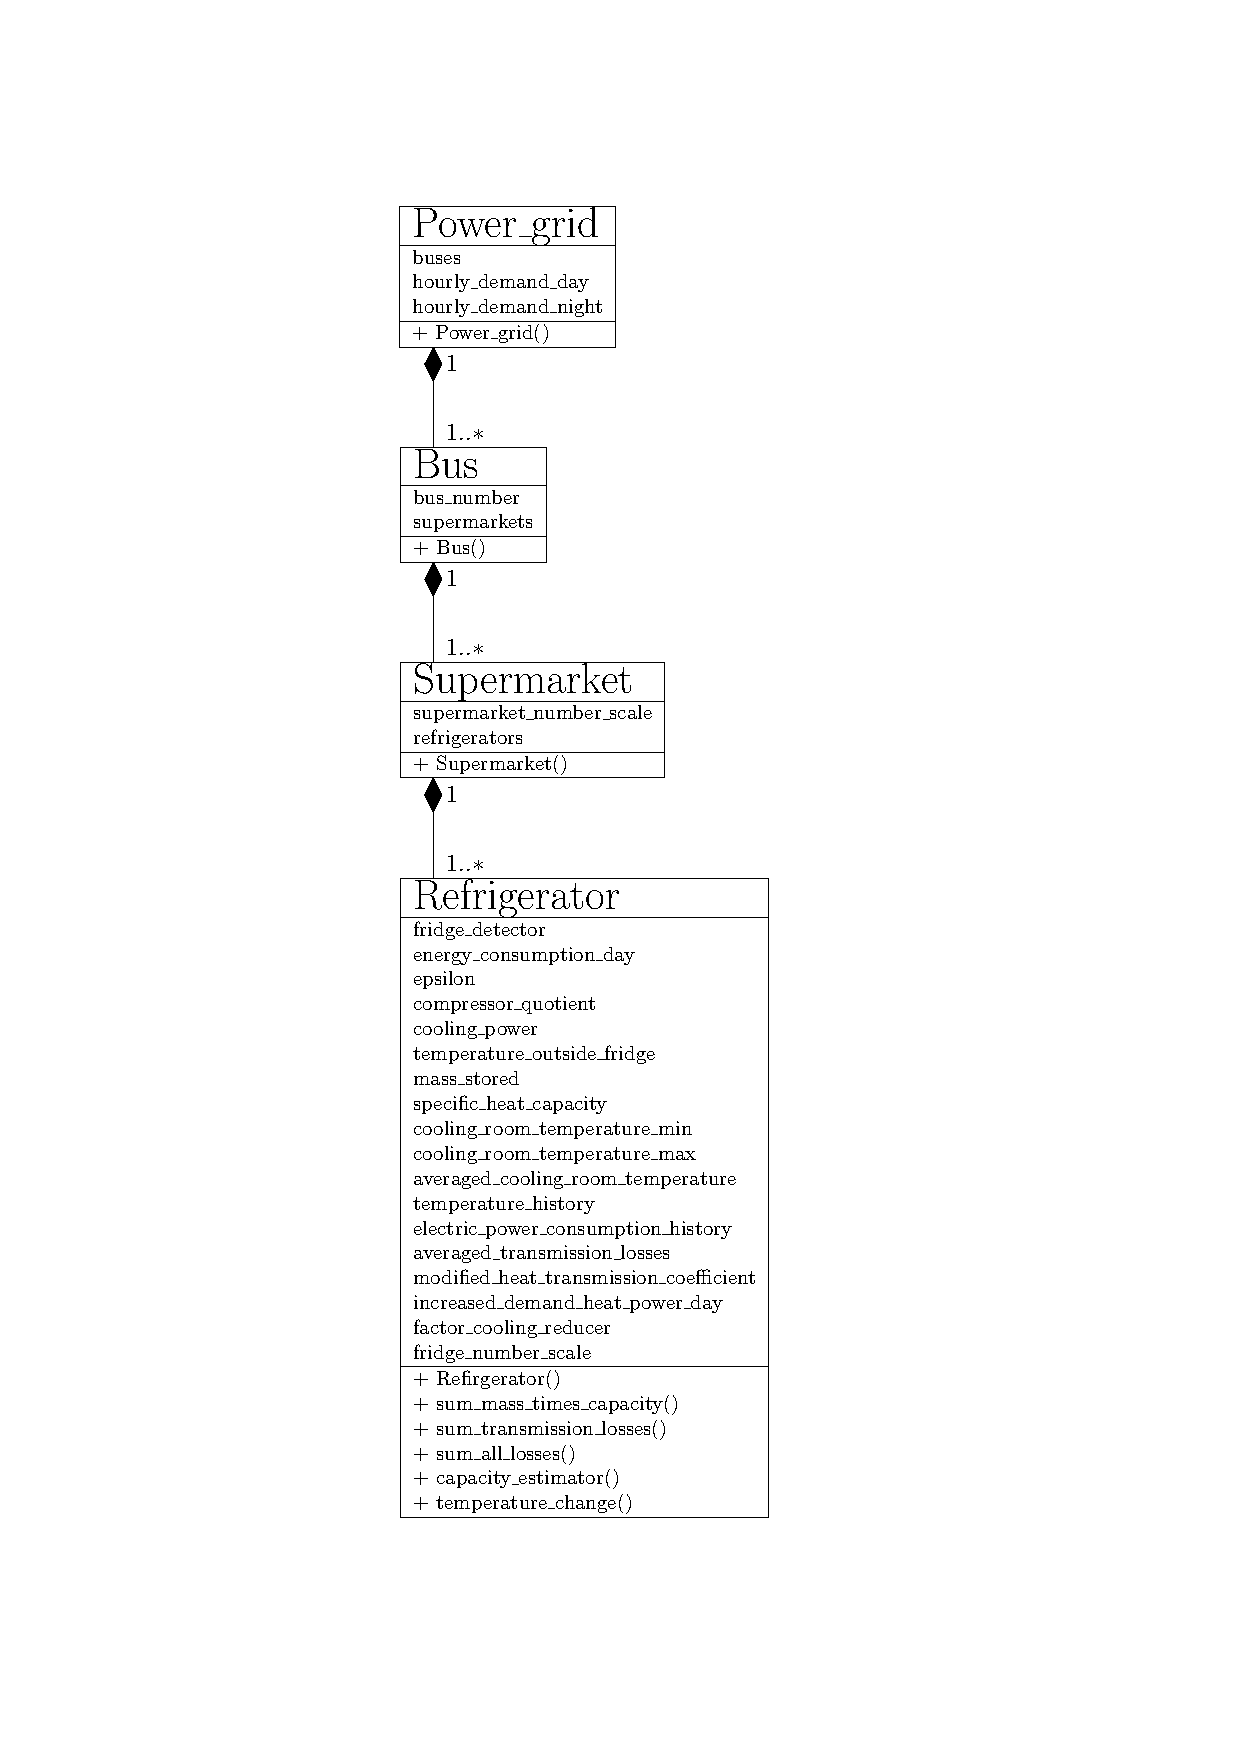
\includegraphics[scale=0.7]{images/Theorie_Super/class_new_diagramm}
	\end{center}
\caption{Klassendiagramm Modellkonstrukt}
\label{fig:klassendiagramm}
\end{figure}

Das Ergebnis der Abstraktion sind vier Klassen. In der Klasse
\textbf{Refrigerator} sind Eigenschaften und Methoden zusammengefasst, die das
Modell einer K\"altelast beschreiben. Darum wird nachfolgend die Klasse
\textbf{Refirgerator} explizit erl\"autert.

\subsection*{Refrigerator}

An dieser Stelle werden die Eigenschaften und die Methoden der Klasse
\textbf{Refrigerator} explizit erkl\"art.

\subsubsection*{Attribute}
\begin{description}
	\item[fridge\_detector] Art der Anlage. Die Berechnung der Verluste der
	Verbundanlagen unterscheidet sich von der der steckerfertigen
	Ger\"ate.
	\item[energy\_consumption\_day] H\"ohe des durchschnittlichen
	elektrischen Energieverbrauchs.
	\item[epsilon] Leistungszahl.
	\item[compressor\_quotient] Anteil des Verdichters am Gesamtverbrauch
	der K\"uhlanlage.
	\item[cooling\_power] K\"alteleistungsbedarf (Herstellerangaben).
	\item[temperatur\_outside\_fridge] $1\times M$-Array mit
	Au\ss entemperaturwertet f\"ur die Umgebung der K\"alteanlage. $M$
	stimmt mit der Anzahl der W\"ande \"uberein, f\"ur die ihre Fl\"ache
	bekannt ist.
	\item[mass\_stored] $1\times N$-Array mit den Massewerten, der zur
	K\"uhlung vorhandenen Substanzmasse. $N$ stimmt mit der Anzahl der
	Massen \"uberein, f\"ur die die spezifische W\"armekapazit\"at
	unterschiedlich ist.
	\item[specific\_heat\_capacity] $1\times N$-Array mit den Werten f\"ur
	spezifische W\"armekapazit\"aten der Substanzmassen.
	\item[cooling\_room\_temperature\_min] Niedrigste Temperatur, die durch
	K\"uhlung erreicht werden darf.
	\item[cooling\_room\_temperature\_max] H\"ochste Temperatur, die durch
	K\"uhlung erreicht werden darf.
	\item[averaged\_cooling\_room\_temperature] Durchschnittliche Temperatur
	im Normalbetrieb.
	\item[temperature\_history] $n \times m$-Array mit $n,m\in
	\mathbb{Z}^+_0$, wobei $n$ f\"ur die Anzahl der Werte des berechneten
	Temperaturverlaufs und $m$ f\"ur die Anzahl der simulierten Tage
	steht. Die Werte sind das Ergebnis der
	Berechnung der Funktion \textbf{main\_equation}. Eine Spalte des Arrays
	stellt den Temperaturverlauf an genau einem Tag dar.
	\item[electric\_power\_consumption\_history] $n \times m$-Array mit
	$n,m\in \mathbb{Z}^+_0$, wobei $n$ f\"ur die Anzahl der Werte des
	berechneten Verbrauchs und $m$ f\"ur die Anzahl der simulierten Tage
	steht. Die Werte sind das Ergebnis der Berechnung der Funktion
	\textbf{main\_equation}. Eine Spalte des Arrays stellt den Verlauf des
	berechneten Verbrauchs an genau einem Tag dar.
	\item[averaged\_transmission\_losses] Summe aller durchschnittlichen
	Transmissionsverluste im Normalbetrieb (vgl. \cref{aptrans} auf der
	Seite \pageref{aptrans}).
	\item[modified\_heat\_transmission\_coefficient] $1\times M$-Array mit
	Werten aus der elementeweisen Multiplikation des Vektors mit den Werten
	der spezifischen W\"armedurchgangskoeffizienten mit dem Vektor mit
	Werten f\"ur die Durchgangsfl\"achen (vgl.  \cref{vmod} auf der Seite
	\pageref{vmod}).
	\item[increased\_demand\_heat\_power\_day] Mehrbedarf am Tag aufgrund
	der zus\"atzlichen Verluste durch Licht, Menschenk\"orperw\"arme,
	T\"ur\"offnungszeiten und weiteren Einfl\"ussen. Die Berechnung erfolgt
	nach einer Auswahl zwischen der \cref{pmehr} und der \cref{lverd} bis
	\cref{spmehr} wie auf den Seiten \pageref{pmehr} und \pageref{spmehr}
	beschrieben.
	\item[factor\_cooling\_reducer] Faktor f\"ur K\"altebedarfsabsenkung
	infolge der Luftfeuchtigkeit und der Umgebungstemperatur.
	\item[fridge\_number\_scale] Anzahl der Anlagen mit der identischen
	technischen Ausf\"uhrung, der Beladung und dem Fahrplan.
\end{description}

\subsubsection*{Methoden}
\begin{description}
	\item[Refrigerator(fridge\_config,number\_steps,days)] Konstruktor der
	Klasse. Bei dem Aufruf dieser Funktion werden folgende Argumente
	\"ubergeben:
	\begin{description}
		\item[fridge\_config] $1 \times 2$-Cell Array
		mit Modellparametern\footnote{ Die Form des Arrays ist
		\"aquivalent zu genau einer Zeile der in
		\matref{csuper} auf der Seite \pageref{csuper} vorgestellten
		Arrays, die die Modelle der Superm\"arkte abbilden.}.
		\item[number\_steps] Anzahl der Zeitschritte, die einen
		Tag beschreiben.
		\item[days] Anzahl der zu simulierenden Tage.
	\end{description}
	Bei der Initialisierung eines Objekts werden einem Teil der oben
	vorgestellten Attribute der Klasse \textbf{Refrigerator} Werte aus dem
	\textbf{ fridge\_config }-Array direkt \"ubergeben. Andere Werte werden
	einmalig von der Konstruktor-Methode berechnet oder im Laufe der
	Simulation ver\"andert.\\

	Folgende Attribute werden einmalig bei der Initialisierung berechnet:
	\begin{description}
		\item[averaged\_transmission\_losses] Summe aller
		durchschnittlichen Transmissionsverluste im Normalbetrieb
		(vgl. \cref{aptrans} auf der Seite \pageref{aptrans}).
		\item[modified\_heat\_transmission\_coefficient] $1\times
		M$-Array mit Werten aus der elementeweisen Multiplikation des
		Vektors mit Werten der spezifischen
		W\"armedurchgangskoeffizienten mit dem Vektor mit den Werten
		f\"ur die Durchgangsfl\"achen (vgl. \cref{vmod} auf der Seite
		\pageref{vmod}).
		\item[increased\_demand\_heat\_power\_day] Mehrbedarf am Tag ,
		aufgrund der zus\"atzlichen Verluste durch Licht,
		Menschenk\"orperw\"arme, T\"ur\"offnungszeiten und weiteren
		Einfl\"usse. Die Berechnung erfolgt nach einer Auswahl
		zwischen der \cref{pmehr} und der \cref{lverd} bis \cref{spmehr}
		wie auf der Seiten \pageref{pmehr} und \pageref{spmehr}
		beschrieben.
	\end{description}

	Folgende Attribute werden im Laufe der Simulation ver\"andert:
	\begin{description}
		\item[temperature\_history] $n \times m$-Array mit $n,m\in
		\mathbb{Z}^+_0$, wobei $n$ f\"ur die Anzahl der Werte des
		berechneten Temperaturverlaufs und $m$ f\"ur die Anzahl der
		simulierten Tage steht. Die Werte sind das Ergebnis der
		Berechnung der Funktion \textbf{main\_equation}. Eine Spalte des
		Arrays stellt den Temperaturverlauf an genau einem Tag dar.
		\item[electric\_power\_consumption\_history] $n \times m$-Array
		mit $n,m\in \mathbb{Z}^+_0$, wobei $n$ f\"ur die Anzahl der
		Werte des berechneten Verbrauchs und $m$ f\"ur die Anzahl der
		simulierten Tage steht. Die Werte sind das Ergebnis der
		Berechnung der Funktion \textbf{main\_equation}. Eine Spalte
		des Arrays stellt den Verlauf des berechneten Verbrauchs an
		genau einem Tag dar.
	\end{description}

	Folgende Attribute sind aufgrund der Annahmen dieser Studie konstant,
	k\"onnen aber bei der einer Modifizierung der Annahmen im Laufe der
	Simulation ver\"andert werden:
	\begin{description}
		\item[temperature\_outside\_fridge] Befindet sich der
		K\"altespeicher au\ss erhalb geschlossener R\"aume und im
		direkten Kontakt mit der Au\ss entemperatur, muss die
		Temperatur\"anderung die im Tagesverlauf in Abh\"angigkeit von
		der Jahreszeit entsteht, beachtet werden.
		\item[mass\_stored] Wenn nicht mehr Angenommen wird, dass
		die Substansmasse im Supermarkt im Laufe des Tages konstant ist,
		sondern mit dem Konsumverhalten der Bev\"olkerung in
		Abh\"angigkeit steht, muss eine Anpassung erfolgen.
	\end{description}

	\item[sum\_mass\_times\_capacity()] Der R\"uckgabewert dieser Funktion
	ist die berechnete Summe aus der elementeweisen Multiplikation aller
	Substanzmassen mit den jeweiligen spezifischen W\"armekapazit\"aten. Der
	Funktion werden keine explizite Argumente \"ubergeben. Die Funktion
	greift direkt auf die Attribute \textbf{specific\_heat\_capacity} und
	\textbf{mass\_stored} des Objekts zu.

	\item[sum\_transmission\_losses()] Es gibt zwei R\"uckgabewerte dieser
	Funktion. Der erste Wert ist die Summe der Transmissionsverluste (vgl.
	\cref{aptrans} auf der Seite \pageref{ptrans}) durch alle
	Durchgangsfl\"achen f\"ur den aktuellen Zeitpunkt und f\"ur die aktuelle
	K\"uhlraumtemperatur. Desweiteren wird die Summe der
	Transimissionsverluste berechnet, die bei der oberen Grenze des
	zugelassenen Temperaturbereichs entsteht. Die Kenntnis hinsichtlich
	dieser Verluste ist wichtig, um die Zeitspanne absch\"atzen zu k\"onnen
	bis die obere Temperaturgrenze erreicht wird (vgl. \cref{tauk} auf der
	Seite
	\pageref{tauk}).

	Die \"Ubergabe folgender Argumente an die Funktion ist erforderlich:
	\begin{description}
		\item[number\_steps] Laufvariable. Gesamtzahl der zu
		simulierenden Zeitschritte f\"ur einen Tag.
		\item[count\_number\_steps] Der aktuelle Wert von
		\textbf{number\_steps}.
		\item[count\_number\_day] Der aktuelle Wert von der Laufvariable
		\textbf{number\_days}.
	\end{description}

	\item[sum\_all\_losses()] Es gibt zwei R\"uckgabewerte dieser Funktion.
	Der erste R\"uckgabewert beinhaltet die Summe aller Verluste an K\"alte
	(vgl. \cref{qv} auf der Seite \pageref{qv}).
	Au\ss erhalb der \"Offnungszeiten entf\"allt der Anteil an
	zus\"atzlichen Verlusten, die durch Licht, offene T\"uren etc.
	anfallen. Durch eine alternative Verzweigung, deren Bedingung die
	Zugeh\"origkeit des aktuellen Wertes der Laufvariable
	\textbf{count\_number\_steps} zu den \"Offnungszeiten ist, wird die
	Ber\"ucksichtigung der zus\"atzlichen Verluste sichergestellt. Der
	zweite R\"uckgabewert ist die Zeitspanne bis zum Erreichen der
	kritischen maximalen Temperatur (vgl. \cref{tauk} auf der Seite
	\pageref{tauk}).

	Die \"Ubergabe folgender Argumente an die Funktion ist erforderlich:
	\begin{description}
		\item[number\_steps] Laufvariable. Gesamtzahl der zu
		simulierenden Zeitschritte f\"ur einen Tag.
		\item[count\_number\_steps] Der aktuelle Wert von
		\textbf{number\_steps}.
		\item[count\_number\_day] Der aktuelle Wert von der Laufvariable
		\textbf{number\_days}.
		\item[number\_days] Laufvariable. Gesamtzahl der zu
		simulierenden Tage.
	\end{description}

	\item[capacity\_estimator()] Die Funktion hat einen R\"uckgabewert.
	Berechnet wird die maximal abzuf\"uhrende W\"armeenergiemenge $\emax$
	(vgl. die \cref{emax} auf der Seite \pageref{emax}).

	Die \"Ubergabe folgender Argumente an die Funktion ist erforderlich:
	\begin{description}
		\item[count\_number\_steps] Der aktuelle Wert von
		\textbf{number\_steps}.
		\item[count\_number\_day] Der aktuelle Wert von der Laufvariable
		\textbf{number\_days}.
		\item[Q\_losses] Wert der aktuellen Verlustk\"altemenge als
		Ergebnis der Funktion \textbf{sum\_all\_losses()} (vgl.
		\cref{qv} auf der Seite \pageref{qv}).
	\end{description}
	\item[temperature\_change()] Die Funktion hat einen R\"uckgabewert.
	Berechnet wird die Temperatur der Substanzmasse, die durch K\"uhlung am
	Ende eines Zeitschritts erreicht wird (vgl. die \cref{tns} auf der
	Seite \pageref{tns}).
	
	Die \"Ubergabe folgender Argumente an die Funktion ist erforderlich:
	\begin{description}
		\item[number\_steps] Laufvariable. Gesamtzahl der zu
		simulierenden Zeitschritte f\"ur einen Tag.
		\item[count\_number\_steps] Der aktuelle Wert von
		\textbf{number\_steps}.
		\item[count\_number\_day] Der aktuelle Wert von der Laufvariable
		\textbf{number\_days}.
		\item[Q\_losses] Wert der aktuellen Verlustk\"altemenge als
		Ergebnis der Funktion \textbf{sum\_all\_losses()} (vgl.
		\cref{qv} auf der Seite \pageref{qv}).
	\end{description}
\end{description}

Alle Klassen haben einen unterschiedlichen Status. Die Klasse
\textbf{Power\_grid} vertritt die Rolle des ganzen Systems, also des
Energieversorgungsnetzes, welches sich aus den charakteristischen Teilen, den
Knoten (\textbf{Bus}) zusammensetzt. Die Existenz eines Knotens au\ss erhalb
eines Netzes ergibt keinen Sinn. Dieser Zusammenhang zwischen Klassen wird im
Klassendiagramm in der \cref{fig:klassendiagramm} durch eine
Linienverbindung/Komposition verdeutlicht.  Auf der Seite des Ganzen endet die
Linie mit einem ausgef\"ullten Rhombus. Das komplette Modell ist nach diesem
Prinzip aufgestellt. Das kleinste Element des Ganzen stellt die K\"alteanlage
(\textbf{Refrigerator}) dar.

\begin{figure}[h]
	\begin{center}
		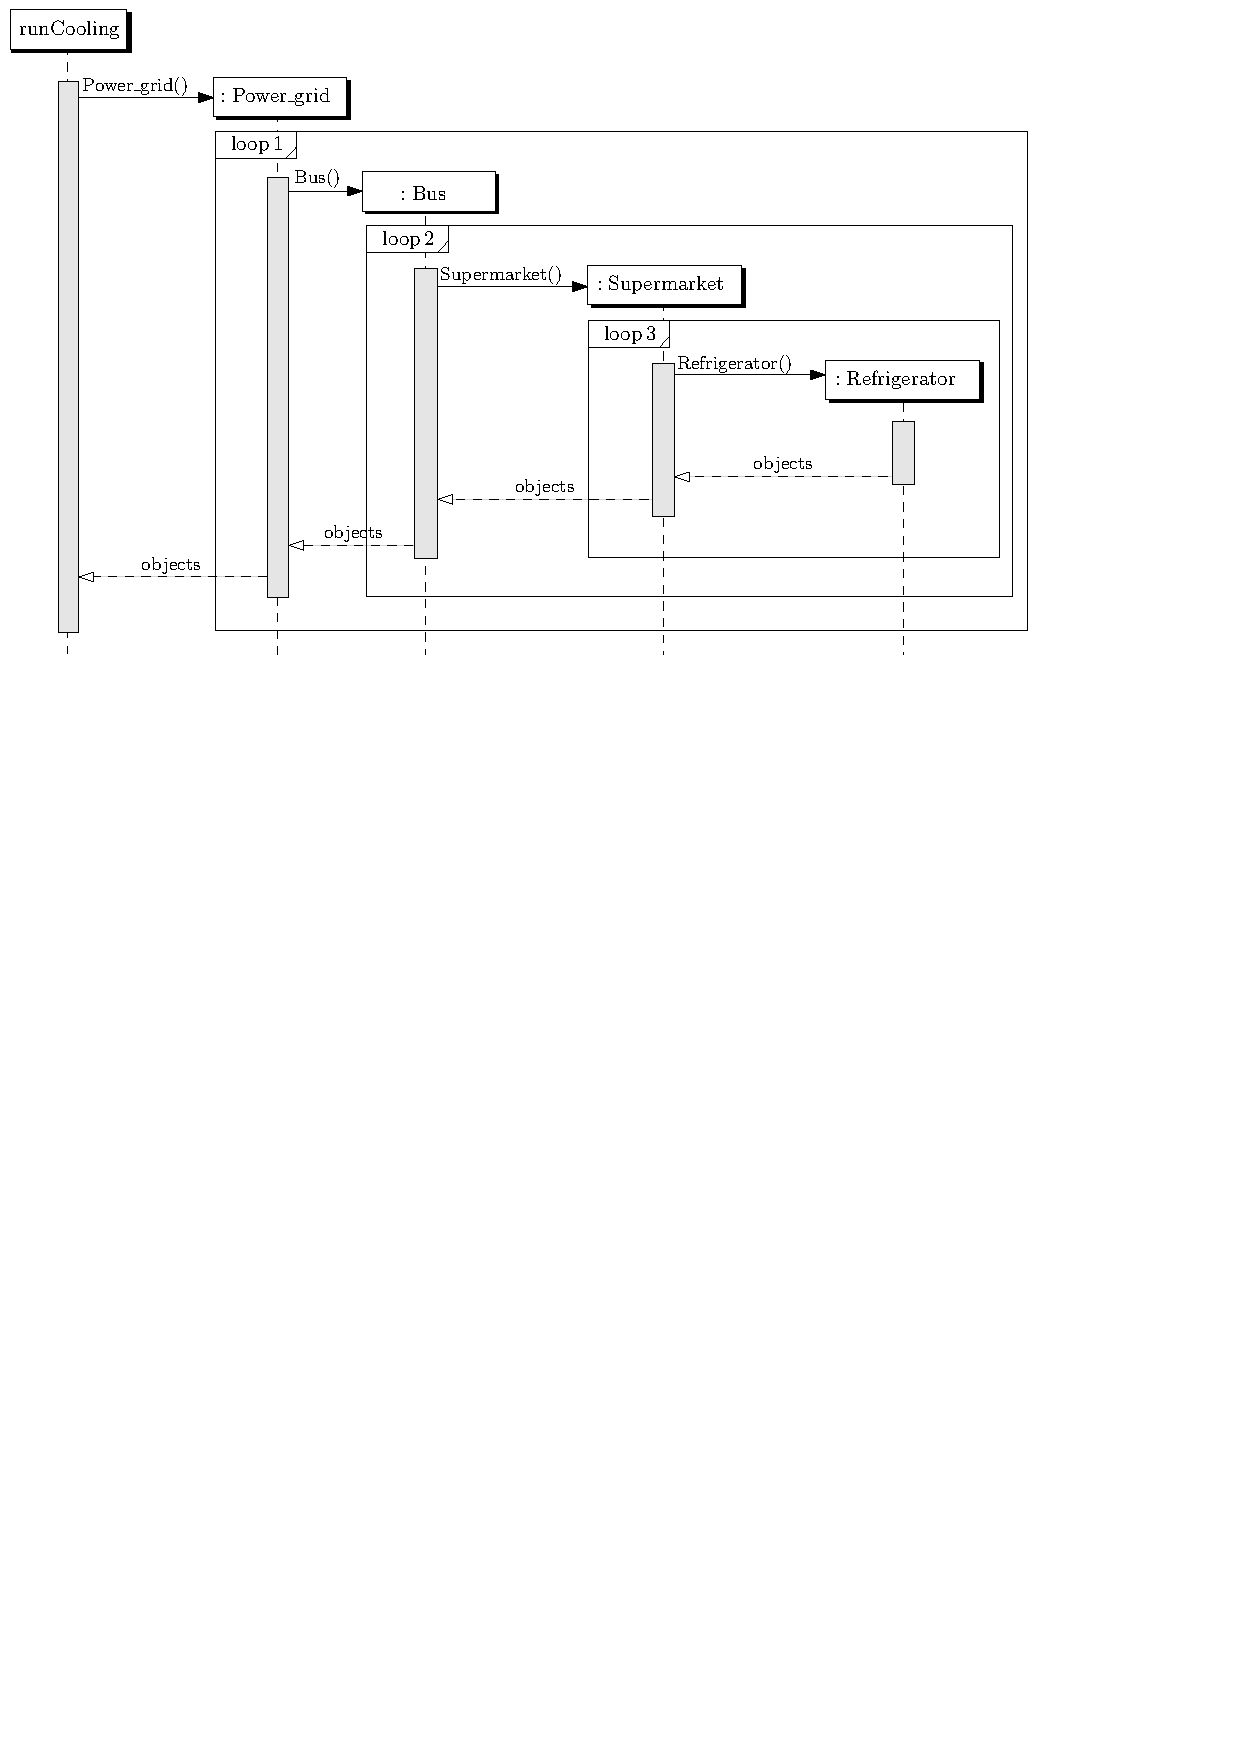
\includegraphics[scale=0.8]{images/Theorie_Super/sequence_one}
	\end{center}
\caption{Sequenzdiagramm Modellkonstrukt}
\label{fig:uml_sequence}
\end{figure}

Aufgrund des Modells wird das elektrische Verhalten einer
Supermarkt-K\"altelast im Energieversorgungsnetz durch miteinander
kooperierende Objekte dargestellt. Wird eine Funktion aufgerufen, die den Start
der Simulation veranlasst, m\"ussen die Objekte aus der Konfigurationsdatei
erzeugt werden.

In der \cref{fig:uml_sequence} auf der Seite \pageref{fig:uml_sequence} wird mit
Hilfe eines Sequenzdiagramms der Nachrichtenaustausch hervorgehoben, der bei
der Erstellung der Objekte durchlaufen wird. Auf der Zeitachse, die senkrecht
von oben nach unten verl\"auft, wird mit Hilfe der Pfeile der Zugriff auf die
Methoden der Objekte hingewiesen. Ist eine Methode des Objekts f\"ur einen
Zeitraum aktiv, wird dieser Zustand durch einen grauen Balken auf dem Zeitstrahl
des zugeh\"origen Objekts visualisiert. Der Aufruf der Funktionen der Objekte
wird durch einen Pfeil mit ausgef\"ullter Spitze dargestellt. Der Pfeil geht vom
Zeitstrahl eines Objekts aus, der die Funktion aufruft und endet mit der Spitze
im Objekt, zu dem diese Funktion geh\"ort. Der Name der aufgerufenen Funktion
steht \"uber dem Pfeil. Wird von dieser Funktion etwas zur\"uckgegeben, so ist
der Pfeil gestrichelt. Die R\"uckgabewerte stehen \"uber dem Pfeil.

In der Funktion \textbf{runCooling}, die den Start der Simulation veranlasst und
steuert, wird der Konstruktor der Klasse \textbf{Power\_grid} aufgerufen. Als
Ergebnis des Aufrufs bekommt die Funktion \textbf{runCooling} ein Objekt der
Klasse \textbf{Power\_grid} mit allen Unterobjekten, die den zu simulierenden
Fall beschreiben. Die Konstruktor-Funktionen der Klassen, die einen
untergeordneten Status besitzen, werden bei der Erstellung der \"ubergeordneten
Objekte aufgerufen. Die Anzahl der erzeugten Objekte h\"angt davon ab, wie oft
die Konstruktor-Funktion der jeweiligen Klasse aufgerufen wird. Diese Zahlen
werden in Konfigurationsdateien abh\"angig von dem untersuchten Fall festgelegt.
Die ausf\"uhrliche Erkl\"arung der Konfigurationsdateien findet im
\cref{sc:handhabung} statt.

\subsection*{Bereitstellung der Leistung zur K\"alteerzeugung}

Das augenblickliche Gleichgewicht zwischen dem K\"altebedarf und der zur
Verf\"ugung stehenden K\"alteleistung sichert die Einhaltung der Soll-Temperatur
der K\"uhlg\"uter. Werden die K\"alteanlagen als Energiespeicher zur Regelung
eingesetzt, so f\"uhrt das, aufgrund der fluktuierenden zur Verf\"ugung
stehenden K\"alteleistung, zu Temperaturschwankungen. Die engen Grenzen des
zul\"assigen Temperaturbandes d\"urfen nicht \"uberschritten werden.

Verschiedene Konzepte f\"ur den Einsatz der K\"alteanlagen als Energiespeicher
im Energieversorgungsnetz sind denkbar.

Im folgenden Abschnitt wird die Implementierung eines m\"oglichen
Kooperationskonzepts zwischen einer Supermarktkette und einem Windpark
vorgestellt.

Die prognostizierten und die tatsächlich vom Windpark produzierten elektrischen
Windleistungsdaten der Vattenfall-Regelzone (heute 50Hertz-Regelzone) aus dem
Jahr 2005 werden als Grundlage-Datensatz verwendet. Im Datensatz sind
Stundenwerte von Windleistung gespeichert, weshalb in diesem Fall auch von
Energie gesprochen werden kann.

Der Windpark ist bestrebt, die Verpflichtung \"uber die Bereitstellung von
Leistung beim Netzbetreiber zu erf\"ullen. Abweichungen, die aufgrund der
fehlerhaften Windprognosen entstehen, sollen durch die Kooperation mit
Supermarktketten ausgeglichen werden.

Es wird angenommen, dass der Prognosefehler von der Windleistungsvorhersage
f\"ur 24 Stunden den 15 \% entspricht. Der Windparkbetreiber meldet beim
Netzbetreiber die untere Grenze an, also 85 \% von der Windleistungsvorhersage.
Der Supermarkt weist einen st\"undlichen Bedarf auf, der unbedingt gedeckt
werden muss. Ist der st\"undliche Bedarf gr\"o\ss er als 15 \% der Prognose,
wird die Differenz aus dem Netz gezogen. Diese Abweichung wird beim
Netzbetreiber zur Erstellung des Lastfahrplans mitgeteilt. Gibt es eine
Abweichung von der
Prognose, so versucht der Supermarkt diese zu absorbieren.

Die vom Windparkbetreiber dem Supermarkt versprochene Leistung wird berechnet,
indem von der Windleistungsvorhersage die 15 \% bestimmt werden oder nur der
st\"undliche Bedarf, wenn er kleiner als die 15 \% ist.
\begin{equation}
	P_{sm} = \min \{ 0,15 \cdot P_{DA},\, P_{dem} \} 
	\label{eq:psm}
\end{equation}

\begin{description}[\dth]
	\item[$P_{sm}$] Leistung, die vom Windparkbetreiber dem Supermarkt
	versprochen wird in MW
	\item[$P_{DA}$] Vorhersage der Windleistung (day ahead) in MW
	\item[$P_{dem}$] St\"undlicher Leistungsbedarf des Supermarkts (demand)
	MW
\end{description}
\vspace{0.5cm}

Die vom Windparkbetreiber beim Netzbetreiber anzumeldende Leistung wird
berechnet, indem von der Windleistungsvorhersage die 85\,\% bestimmt werden
oder der st\"undliche Bedarf des Supermarkts abgezogen wird, wenn er kleiner
als die 15\,\% ist.
\begin{equation}
	P_{net} = P_{DA} - P_{sm}
	\label{eq:pnet}
\end{equation}

\begin{description}[\dth]
	\item[$P_{net}$] Leistung, die vom Windparkbetreiber beim Netzbetreiber
	angemeldet wird in MW
	\item[$P_{DA}$] Vorhersage der Windleistung (day ahead) in MW
	\item[$P_{dem}$] St\"undlicher Leistungsbedarf des Supermarkts (demand)
	MW
 \end{description} \vspace{0.5cm}


Die Leistung, die insgesamt den K\"alteanlagen zur Verf\"ugung steht, berechnet
sich nach der \cref{pload}. Der Ausdruck $P_{RT} - P_{net}$ bedeutet die
\"ubersch\"ussige Windleistung. Der Ausdruck $P_{dem} - P_{sm}$  bedeutet die
vom Supermarkt beim Netzbetreiber nicht abgemeldete Leistung.

\begin{align}
	P_{load} &= P_{RT} - P_{net} + P_{dem} - P_{sm}\\
		&= P_{RT} - P_{DA} + P_{dem}
	\label{pload}
\end{align}
\begin{description}[\dth]
	\item[$P_{load}$] Vorhandene Leistung zum Laden in MW
	\item[$P_{RT}$] Windleistungsdaten. Windleistung, die tats\"achlich vom
	Windpark generiert wurde in MW
	\item[$P_{net}$] Leistung, die vom Windparkbetreiber beim Netzbetreiber
	angemeldet wird in MW
	\item[$P_{dem}$] St\"undlicher Leistungsbedarf des Supermarkts (demand)
	\item[$P_{sm}$] Leistung, die vom Windparkbetreiber dem Supermarkt
	versprochen wird in MW
\end{description} \vspace{0.5cm}

\subsubsection*{Implementierung}
Die Implementierung des Kooperationskonzepts erfolgt in einer neuen Klasse
\textbf{Cooling\_strategy}. Diese Klasse hat die Aufgabe, jeder K\"uhlstelle in
jedem Supermarkt im Netz die aufgrund des Kooperationskonzepts und der
Temperaturbeschr\"ankungen optimale Menge an K\"alteleistung zuzuweisen. Die zur
Verf\"ugung stehende Leistung wird auf alle K\"uhlstellen gleichm\"a\ss ig
aufgeteilt bis keine Leistung mehr vorhanden ist oder die Minimaltemperatur
erreicht wird. Alle K\"uhlstellen sollen zu jeder Stunde mindestens soviel
Leistung zugewiesen bekommen, dass genau diese eine Stunde \"uberbr\"uckt werden
kann, ohne, dass die H\"ochsttemperatur \"uberschritten wird. Die Zeit bis zur
H\"ochsttemperatur darf also nie unter eine Stunde fallen. Um diese
Zeitbeschr\"ankung zu erf\"ullen, muss ermittelt werden, ob die verbleibende
Zeit bis zur oberen Schranke nicht unter eine Stunde f\"allt, wenn keine
K\"uhlleistung vorhanden ist.
Diese Zeit kann nach der \cref{tauk} abgesch\"atz werden.
\begin{align}
	\tau_{krit}(i) &= \frac{m \cdot c \cdot (t_{max} -
		t(i))}{Q_{v_{ln}}(i)}
\label{tauk}
\end{align}
\begin{align*}
	Q_{v_{ln}}(i) &= \begin{cases}
	1h \cdot \aptranslog(i), & \text{au\ss erhalb der \"Offnungszeiten}\\
	1h \cdot (\aptranslog(i) + \pmehr(i)), & \text{innerhalb der
	\"Offnungszeiten} \end{cases}
\end{align*}

\begin{description}[\dth]
	\item[$Q_{v_{ln}}(i)$] Verlustk\"altemenge zur Stunde $i$ in kJ
	\item[$\tau_{krit}(i)$] Zeit bis zur kritischen Temperatur zur Stunde
	$i$ in h
	\item[$m$] Substanzmasse zur Aufnahme der Wärmeenergie in kg
	\item[$c$] Spezifische Wärmekapazität der Substanzmasse in $\mathrm{\frac{kJ}{kg
		\cdot K}}$
	\item[$t_{max}$] Obere Temperaturgrenze in $ ^{\circ} $C
	\item[$t(i)$] Temperatur zur Stunde $i$ in $ ^{\circ} $C
	\item[$\aptranslog(i)$] Logarithmierter Mittelwert der
		Transmissionswärmeleistung zum aktuellen Zeitpunkt in kW
	\item[$\pmehr(i)$] Tagesmehrbedarf zum aktuellen Zeitpunkt in kW
\end{description}
\vspace{0.5cm}
Die Differenz zwischen der Transmissionswärmeleistung f\"ur den aktuellen
Zeitpunkt wenn die K\"uhlraumtemperatur minimal w\"are, und der
Transmissionswärmeleistung zum aktuellen Zeitpunkt geteilt durch den Logarithmus
aus der Division der beiden Leistungen, ergibt den logarithmierten Mittelwert
der Transmissionswärmeleistung.
\begin{equation}
	\aptranslog(i) = \frac{ \ptransm(i) - \ptrans(i) }{\log \left(
		\frac{\ptransm(i)}{\ptrans(i)} \right)}
	\label{log}
\end{equation}

\begin{description}[\dth]
	\item[$\aptranslog(i)$] Logarithmierter Mittelwert der
		Transmissionswärmeleistung zum aktuellen Zeitpunkt in kW
	\item[$\ptransm(i)$] Transmissionswärmeleistung f\"ur den aktuellen
	Zeitpunkt, wenn die K\"uhlraumtemperatur minimal w\"are in kW
	\item[$\ptrans(i)$] Transmissionswärmeleistung f\"ur den aktuellen
	Zeitpunkt  kW
\end{description}
\vspace{0.5cm}

\begin{equation}
	\ptransm(i) = A \cdot k \cdot \left( t_{max} -
	t(i) \right)
	\label{ptransmi}
\end{equation}

\begin{description}[\dth]

	\item[$\ptransm(i)$] Transmissionswärmeleistung f\"ur den aktuellen
	Zeitpunkt, wenn die K\"uhlraumtemperatur minimal w\"are in kW
	\item[$A$] Fläche in $\mathrm{m^2}$
	\item[$k$] Wärmedurchgangskoeffizient in $\mathrm{\frac{W}{m^2 \cdot
	K}}$
	\item[$t_{max}$] Obere Temperaturgrenze in $ ^{\circ} $C
	\item[$t(i)$] Temperatur zur Stunde $i$ in $ ^{\circ} $C
\end{description}
\vspace{0.5cm}

\begin{equation}
	\ptrans(i) = A \cdot k \cdot \left( t_{amb}(i) -
	t(i) \right)
	\label{ptransi}
\end{equation}

\begin{description}[\dth]

	\item[$\ptrans(i)$] Aktuelle Transmissionswärmeleistung in kW
	\item[$A$] Fläche in $\mathrm{m^2}$
	\item[$k$] Wärmedurchgangskoeffizient in $\mathrm{\frac{W}{m^2 \cdot
	K}}$
	\item[$t_{amb}(i)$] Aktuelle Umgebungstemperatur in $^{\circ}$C
	\item[$t(i)$] Aktuelle Kühlraumtemperatur in $^{\circ}$C
\end{description}
\vspace{0.5cm}

Um den Temperaturausgleich bei den Lebensmitteln im Algorithmus zu
berücksichtigen, werden deshalb die zu- und abgeführten Wärmeenergiemengen bei
der Berechnung der Temperatur für jeden Zeitschritt stets mit dem Faktor 0,8
multipliziert.  Die Gleichung zur stündlichen Berechnung der aktuellen
Temperatur ist damit:

\begin{equation}
	t(i+1) = 0.8 \cdot \frac{Q_v - Q_{ab}}{m \cdot c}h + t(i)
\label{tns}
\end{equation}

\begin{description}[\dth]

	\item[$t$] Temperatur in $^{\circ} $C
	\item[$Q_v$] Eindringende Verlustwärmemenge in kJ
	\item[$Q_{ab}$] Abführende Wärmemenge in kJ

\end{description}
\vspace{0.5cm}

wobei $Q_v$ die aktuell eindringende Wärmeenergie und $Q_{ab}$ die abgeführte
Wärmeenergie ist.

\begin{figure}[h!]
	\begin{center}
	\includegraphics[scale=0.7]{images/Theorie_Super/class_diagramm_second}
	\end{center}
\caption{Klassendiagramm Kooperationskonzept}
\label{fig:klasskoop}
\end{figure}

In der \cref{fig:klasskoop} auf der Seite \pageref{fig:klasskoop} wird in einem
Klassendiagramm die Beziehung zwischen dem bestehenden Modell und der Klasse
\textbf{Cooling\_strategy} veranschaulicht. Eine Klasse
\textbf{Cooling\_strategy} steht in der direkten Verbindung mit der Klasse
\textbf{Refrigerator}, f\"ur die sie die zur K\"uhlung erforderliche Leistung
berechnet. Ein Objekt der Klasse \textbf{Cooling\_strategy} kann mit einem bis
mehreren Objekten der Klasse \textbf{Refrigerator} in Verbindung stehen.\\

In der \cref{fig:coop} auf der Seite \pageref{fig:coop} ist der
Programmstrukturplan des Kooperationskonzepts abgebildet. Der Algorithmus
zeigt den Ablauf beim "`Auff\"ullen"' der K\"uhlstellen  f\"ur genau einen
Zeitschritt der Simulation. Die Umsetzung des Algorithmus erfolgt
in der Funktion \textbf{strategy\_calculator()}.

\begin{description}
\item[strategy\_calculator()] Es gibt f\"unf R\"uckgabewerte dieser Funktion.
Der erste R\"uckgabewert ist ein $n\times11\,$-Array, wobei $n$ f\"ur die Anzahl
der im gesamten Netz vorhandenen K\"uhlzellen steht. Dieser Array wird zu jedem
Zeitschritt (Stunde) der Simulation neu erzeugt. In den Spalten des Arrays
werden alle Informationen gespeichert, die durch Berechnungen in der Funktion
entstanden sind und weitere Informationen, die zur eindeutigen Zuordnung dieser
Ergebnisse zu der jeweiligen K\"alteeinheit beitragen. Die Energie zum K\"uhlen
wird f\"ur die jeweiligen K\"uhleinheiten z.B. in der Spalte sechs gespeichert.
Der zweite Ausgabewert ist der st\"undliche Leistungbedarf $P_{dem}$ f\"ur das
Gesamtnetz.  Die f\"ur das Gesamtnetz berechnete vorhandene Leistung zum Laden
$P_{load}$ ist der dritte Ausgabewert. Der vierte Wert ist die vom
Windparkbetreiber beim Netzbetreiber angemeldete Leistung $b$ f\"ur das
Gesamtnetz. Der f\"unfte Ausgabewert ist die dem Supermarkt vom
Windparkbetreiber versprochene Leistung.  Die letzten drei Ausgaben berechnen
sich nach den Formeln, die in der \cref{pload} auf der Seite \pageref{pload} zu
sehen sind.

Die \"Ubergabe folgender Attribute an die Funktion ist erforderlich.

\begin{description} 
\item[buses] Referenz zum Attribut \textbf{buses} vom Objekt der Klasse
\textbf{Power\_grid}
\item[hourly\_demand\_day] Referenz zum Attribut \textbf{hourly\_demand\_day}
vom Objekt der Klasse \textbf{Power\_grid}
\item[hourly\_demand\_night] Referenz zum Attribut
\textbf{hourly\_demand\_night} vom Objekt der Klasse \textbf{Power\_grid}
\item[count\_number\_day] Der aktuelle Wert von der Laufvariable number\_day
\item[count\_number\_steps] Der aktuelle Wert von der Laufvariable number\_steps
\item[gen\_out\_day\_T] Daten der tats\"achlich vom Windpark generierten
Leistung f\"ur den untersuchten Zeitraum
\item[gen\_out\_day\_A] Windleistungsprognosedaten f\"ur den untersuchten Zeitraum
\item[promised\_gen\_output\_DA\_gros] untere Grenze des angenommenen Bandes
f\"ur Abweichung der Windleistungsprognosedaten von realen Werten f\"ur den
untersuchten Zeitraum
\item[number\_day] Laufvariable. Gesamtzahl der zu simulierenden Tage.
\item[number\_steps] Laufvariable. Gesamtzahl der zu simulierenden Zeitschritte
f\"ur einen Tag.  \end{description}

\end{description}

Der Auff\"ullvorgang findet zwischen den st\"undlichen Temperaturberechnungen
statt. Diese Handlung wird schrittweise wiederholt, um die gleichm\"a\ss ige
Verteilung der Leistung auf alle Anlagen zu erm\"oglichen. Zur L\"osung dieser
Aufgabe im Programm ist eine \textbf{while}-Schleife mit einer Abbruchbedingung
geeignet. Innerhalb der \textbf{while}-Schleife wird der Algorithmus, der in
der \cref{fig:coop} zu sehen ist, umgesetzt.

Im ersten Schritt des Algorithmus findet eine Abfrage statt, ob Leistung zum
K\"uhlen der Anlagen zur Verf\"ugung steht. Der Abfrage liegt eine Berechnung
(vgl. \cref{pload} auf der Seite \pageref{pload}) zugrunde, die in der
Funktion \textbf{power\_for\_load\_net()} implementiert ist.

\begin{description}
\item[Fall 1] Die Menge der Leistung ist nicht gr\"o\ss er Null. Es erfolgt die
n\"achste Abfrage nach den K\"uhlstellen, die eine Stunde ohne Leistung aus dem
Netz nicht \"uberstehen k\"onnen, ohne die kritische Temperatur zu
\"uberschreiten.  Diese Anlagen werden mit der zus\"atzlichen, nicht
angemeldeten Leistung aus dem Netz geladen, sodass sie genau eine Stunde
\"uberstehen, ohne die obere Temperaturgrenze zu verletzen. Der Vorgang endet
anschlie\ss end, und es kann zum n\"achsten Zeitschritt der Simulation
\"ubergegangen werden.

Sind keine solche K\"uhlstellen vorhanden, endet der Vorgang und es kann zum
n\"achsten Zeitschritt der Simulation \"ubergegangen werden.

\item[Fall 2] Die Menge der Leistung ist gr\"o\ss er Null. In diesem Fall werden
alle K\"uhlstellen gefunden, deren Kapazit\"at (vgl. die \cref{eq:ap}) noch
nicht ausgesch\"opft ist und deren Zeit bis zum Erreichen der kritischen
Temperatur am kleinsten ist.  Anschlie\ss end wird \"uberpr\"uft, ob eine
W\"armeenergie abgef\"uhrt werden kann, die genau $\frac{1}{60}\cdot
Q_v$\footnote{ $Q_v$ ist die eindringende Verlustw\"armemenge in kJ.}
entspricht, ohne als Folge die \"Uberschreitung der minimalen Temperatur zu
verursachen. Ist das der Fall, wird die Kapazit\"at dieser K\"uhlstelle gleich
Null gesetzt, damit diese K\"uhlstelle beim n\"achsten Durchgang der
\textbf{while}-Schleife nicht beachtet wird.

Ist das Abf\"uhren der W\"armeenergiemenge ohne Verletzung der Temperaturgrenzen
m\"oglich, so wird anschlie\ss end die Kapazit\"at, die zur Verf\"ugung
stehende Gesamtleistung und die Leistung, die zur K\"uhlung dieser K\"uhltruhe
bereitgestellt wird, um diese Leistungsmenge erg\"anzt. Die Zeit $\tau_{krit}$
wird um einen Zeitschritt erg\"anzt. Der Zyklus der \textbf{while}-Schleife
setzt sich fort.
\begin{equation}
	Q_{Kap} = Q_{max} - \frac{1}{60}Q_v\\
	\label{eq:ap}
\end{equation}
\begin{equation*}
	P_{load} = P_{load} - \frac{1}{60}\frac{Q_v }{3,6 \cdot 10^{6} \cdot
	\epsilon}
\end{equation*}
\begin{equation*}
	\tau_{krit} = \tau_{krit} + \frac{1}{60}
\end{equation*}
\begin{equation*}
	Q_{cooling} = Q_{cooling} + \frac{1}{60}Q_v
\end{equation*}
\begin{description}[\dth]
\item[$Q_{Kap}$] W\"armeenergiemenge, die zus\"atzlich abgef\"uhrt werden kann,
ohne dass die minimale Temperaturgrenze verletzt wird in kJ
\item[$Q_{max}$] Maximal abzuf\"uhrende W\"armeenergiemenge in kJ
\item[$Q_{v}$] Eindringende Verlustw\"armemenge in kJ
\item[$P_{load}$] Vorhandene Ladeleistung in MW
\item[$\tau_{krit}$] Zeit bis zur kritischen Temperatur in h
\item[$Q_{cooling}$] W\"armeenergiemenge, die der K\"uhlzelle zur K\"uhlung
zugewiesen wird in kJ
\end{description} \vspace{0.5cm}
\begin{equation}
	\emax = m \cdot c \cdot (t(i) - t_{min}) + Q_v
\label{emax}
\end{equation}

\begin{description}[\dth]

	\item[$\emax$] Maximal abzuf\"uhrende W\"armeenergiemenge in kJ
	\item[$m$] Substanzmasse zur Aufnahme der Wärmeenergie in kg
	\item[$c$] Spezifische Wärmekapazität der Substanzmasse in $\mathrm{\frac{kJ}{kg
		\cdot K}}$
	\item[$Q_v$] Verlustk\"altemenge in kJ
	\item[$t_{min}$] Obere Temperaturgrenze in  $\grad$ C
	\item[$t(i)$] Temperatur zur Stunde $i$ in  $\grad$ C

\end{description}
\vspace{0.5cm}

\end{description}

\begin{figure}[h!]
	\begin{center}
	\includegraphics[scale=0.8]{images/Theorie_Super/cooperation}
	\end{center}
\caption{Flussdiagramm}
\label{fig:coop}
\end{figure}

Der genaue Ablauf des Informationsflusses, der zwischen den Objekten im Verlauf
der Simulation des Kooperationskonzepts stattfindet, wird im Sequenzdiagramm in
der \cref{fig:uml_coop} auf der Seite \pageref{fig:uml_coop} grafisch
erl\"autert.
\begin{figure}[h]
	\begin{center}
	\includegraphics[scale=1.15]{images/Theorie_Super/double}
	\end{center}
\caption{Sequenzdiagramm Kooperationsstrategie}
\label{fig:uml_coop}
\end{figure}



%%%%%%%%%%%%%%%%%%%%%%%%%%%%%%%%%%%%%%%%%%%%%%%%%%%%%%%%
%%%%%%%%%%%%%%%%%%%%%%%%%%%%%%%%%%%%%%%%%%%%%%%%%%%%%%%%
\section{Handhabung des Programms}
\label{sc:handhabung}

\subsection{Systemanforderungen}

Zur Benutzung des Programms muss aufgrund der gewählten Programmiersprache und
der objektorientierten Programmierweise folgendes gelten:

\begin{itemize}
	\item Im Rechner muss die Software \matlab der Version $5.0$ oder
	höher\footnote{ \matlab verfügbar über The MathWorks, Inc.
	(http://www.mathworks.com).} eingerichtet sein.
\end{itemize}

Die Anforderungen an die Hardware sind durch die eingesetzte \matlab-Version
bestimmt.

%%%%%%%%%%%%%%%%%%%%%%%%%%%%%%%%%%%%%%%%%%%%%%%%%%%%%%%%
%%%%%%%%%%%%%%%%%%%%%%%%%%%%%%%%%%%%%%%%%%%%%%%%%%%%%%%%
%%%%%%%%%%%%%%%%%%%%%%%%%%%%%%%%%%%%%%%%%%%%%%%%%%%%%%%%
\subsection{Installation}

Das Programm richtet sich in seiner Installation und der Benutzung nach dem
allgemein gültigen Gebrauch der \matlab M-files\footnote{
Ausführliche Information dazu findet man z.B. in \cite{MATLAB-Buch}.}.

%%%%%%%%%%%%%%%%%%%%%%%%%%%%%%%%%%%%%%%%%%%%%%%%%%%%%%%%
%%%%%%%%%%%%%%%%%%%%%%%%%%%%%%%%%%%%%%%%%%%%%%%%%%%%%%%%
%%%%%%%%%%%%%%%%%%%%%%%%%%%%%%%%%%%%%%%%%%%%%%%%%%%%%%%%
\subsection{Aufruf der Simulation}%
%%%%%%%%%%%%%%%%%%%%%%%%%%%%%%%%%%%%%%%%%%%%%%%%%%%%%%%%
%%%%%%%%%%%%%%%%%%%%%%%%%%%%%%%%%%%%%%%%%%%%%%%%%%%%%%%%
%%%%%%%%%%%%%%%%%%%%%%%%%%%%%%%%%%%%%%%%%%%%%%%%%%%%%%%%
\subsection*{Vorbereitung der Input-Information}
\label{sec:input_infos}

Zum Starten des Programms werden folgende Konfigurationsdateien\footnote{ Bei
der Simulation wurden die Konfigurationsdateien verwendet, die im
\matref{crgrid}, \matref{crsuper} und \matref{crfridge}
dargestellt sind.} benötigt:

\begin{itemize}
	\item config\_grid.m
	\item config\_supermarkets.m
	\item config\_fridges.m
\end{itemize}
%%%%%%%%%%%%%%%%%%%%%%%%%%%%%%%%%%%%%%%%%%%%%%%%%%%%%%%%
%%%%%%%%%%%%%%%%%%%%%%%%%%%%%%%%%%%%%%%%%%%%%%%%%%%%%%%%
%%%%%%%%%%%%%%%%%%%%%%%%%%%%%%%%%%%%%%%%%%%%%%%%%%%%%%%%
\vspace{3mm}
\noindent\textbf{config\_grid.m}
\vspace{3mm}

Es ist wichtig, dass die topologischen Eigenschaften des Netzes im Programm
berücksichtigt werden. Damit das Programm mit den für die Simulation notwendigen
Informationen, die das Energienetz beschreiben, versorgt wird, ist die Form, die
in \matref{cgrid} vorgestellt wird, für die \textbf{config\_grid.m$\,$}-Datei
zwingend:

\begin{lstlisting}[float=h,caption={config\_grid.m},label={cgrid}]
%%	Bus,  Supermarkets,	  Number of Supermarkets
configuration_grid = {...
        1 , {Aldi	     ,	      1500;	     ...
             Netto	     ,	       500};	 ...
        2 , {0	         ,           0};	 ...
        3 , {0	         ,           0};	 ...
        4 , {0	         ,           0}	     ...
       };
\end{lstlisting}

In der \textbf{config\_grid.m}$\,$-Datei wird  ein $n\times2\,$-Cell Array
($n\in \mathbb{Z}^+_0$) definiert, der die Information über die Topologie des
Netzes sowie die Verteilung der Kältelasten im Netz beinhaltet. Ein Cell Array
ist ein Speicherobjekt, der verschiedene Datentypen unterschiedlicher Größe
aufnehmen kann\cite[Teil 2, Seite 15]{MATLAB-Buch}.  Ein Cell Array wird mit dem
Befehl $c=cell(\ldots)$ oder mit Hilfe von geschweiften Klammern $c=\{\ldots\}$,
wie in diesem Fall, erzeugt. Jede Zeile des Cell Arrays
\textbf{configuration\_grid}, der in der \textbf{config\_grid.m}$\,$-Datei
definiert werden muss, steht für ein Knotenpunkt im Netz. In der ersten Spalte
wird die Nummer des Knotens bzw. Busses gespeichert. In die zweite Spalte
werden die Arten der Kältelasten und deren Anzahl am jeweiligen Knoten
festgelegt. Es ist wiederum ein $m\times2\,$-Cell Array ($m\in \mathbb{Z}^+_0$).
Jede Zeile dieses Cell Arrays ist für eine eigene Art Supermarktkette
reserviert. In die erste Spalte kommt der Name der Supermarktkette deren
Eigenschaften in der \textbf{config\_supermarkets.m$\,$}-Datei (vgl.
\matref{csuper}) gespeichert sind. In der zweiten Spalte wird die Anzahl der
Supermärkte einer Kette festgelegt, die an dem bestimmten Knoten simuliert
werden soll.

Um Fehler auf dieser Ebene zu vermeiden, muss die
\textbf{config\_grid.m}$\,$-Datei unbedingt die oben vorgestellte Form
beibehalten.

%%%%%%%%%%%%%%%%%%%%%%%%%%%%%%%%%%%%%%%%%%%%%%%%%%%%%%%%
%%%%%%%%%%%%%%%%%%%%%%%%%%%%%%%%%%%%%%%%%%%%%%%%%%%%%%%%
%%%%%%%%%%%%%%%%%%%%%%%%%%%%%%%%%%%%%%%%%%%%%%%%%%%%%%%%
\vspace{3mm}
\noindent\textbf{config\_supermarkets.m}
\vspace{3mm}

%%%%%%%%%%%%%%%%%%%%%%%%%%%%%%%%%%%%%%%%%%%%%%%%%%%%%%%%%%%%%%%%%%%%%%%%%%%%%%%%
% Abkürzungen die config_supermarkets betreffen
\abvz{NK\_KT\_S}{normalgekühlte Kühltruhe steckerfertig}
\abvz{NK\_KR\_V}{normalgekühltes Kühlregal an Verbundanlage}
\abvz{TK\_TKT\_S}{tiefgekühlte Tiefkühltruhe steckerfertig}
\abvz{NK\_KZ}{normalgek\"uhlte K\"uhlzelle an Vergundanlage}
\abvz{TK\_KZ}{tiefgek\"uhlte Tiefk\"uhlzelle K\"alteaggregat}
%%%%%%%%%%%%%%%%%%%%%%%%%%%%%%%%%%%%%%%%%%%%%%%%%%%%%%%%%%%%%%%%%%%%%%%%%%%%%%%%

\begin{lstlisting}[float=h!,caption=config\_supermarkets.m,label={csuper}]
%%       Kind of fridge     Anzahl
Aldi = {...
        { NK_KT_S      ,    1 };     ...
        { NK_KR_V      ,    2 };     ...
        { TK_TKT_S     ,    1 }      ...
       };
Netto = {...
        { NK_KT_S      ,    5 };     ...
       };
\end{lstlisting}

Die Kältelast in einem Supermarkt bilden die einzelnen je nach Einsatzzweck
speziell dafür konstruierten K\"uhleinheiten. Die Anzahl, die technischen
Eigenschaften und die Betriebsweise dieser Kältemaschinen können in der
Realität Unterschiede aufweisen. In der Konfigurationsdatei
\textbf{config\_supermarkets.m$\,$} (vgl. \matref{csuper}) wird festgelegt, wie
die einzelnen Supermarktketten aus verschiedenen Kälteeinheiten zusammengesetzt
sind. Die Gruppierung der einzelnen K\"uhleinheiten zu einem Modellsupermarkt
erfolgt in der \textbf{config\_supermarkets.m$\,$}-Datei durch Definition eines
oder mehrerer $i\times2\,$-Cell ($i\in \mathbb{Z}^+_0$) Arrays, die jeweils
einen Supermarkt abbilden. Jede Zeile eines solchen Cell Arrays ist für je eine
Art K\"uhleinheit reserviert. In die erste Spalte kommt der Name der
K\"uhlzelle, deren Eigenschaften in der \textbf{config\_fridges.m}-Datei (vgl.
\matref{fridge} auf der Seite \pageref{fridge}) gespeichert sind. In der zweiten
Spalte wird die Anzahl f\"ur diese K\"uhleinheiten, die in dem Supermarkt
betrieben werden, festgelegt.

%%%%%%%%%%%%%%%%%%%%%%%%%%%%%%%%%%%%%%%%%%%%%%%%%%%%%%%
%%%%%%%%%%%%%%%%%%%%%%%%%%%%%%%%%%%%%%%%%%%%%%%%%%%%%%%
%%%%%%%%%%%%%%%%%%%%%%%%%%%%%%%%%%%%%%%%%%%%%%%%%%%%%%%
\vspace{3mm}%
\noindent\textbf{config\_fridges.m}
\vspace{3mm}

Die Konfigurationsdatei \textbf{config\_fridges.m} kann als eine Datenbank für
Kälteeinheiten aufgefasst werden. In dieser Datenbank werden Informationen nach
einem bestimmten Muster gruppiert und gespeichert, sodass jede Gruppe eine
bestimmte K\"uhleinheit abbildet. Im Programm kann aus je einem dieser
physikalisch fundierten Modellen ein K\"uhleinheit-Objekt erzeugt werden.

Am Beispiel des Modells einer steckerfertigen Normalkühltruhe, abgekürzt
NK\_KT\_S (vgl. \matref{fridge} auf der Seite \pageref{fridge}), wird im
Folgenden die Eingabeform eines solchen Datenbankeintrages in der Datei
\textbf{config\_fridges.m} erläutert.  Zur Beschreibung einer K\"uhleinheit ist
es erforderlich, die Annahmen in einen $1\times14\,$-Cell Array zu erfassen. Die
Größe und die Art des Arrays ist vorgegeben durch die Auslegung des Modells zur
Anzahl und dem Typus der modellbeschreibenden Annahmen. Die Struktur eines Cell
Arrays ermöglicht neben der zusammenhängenden Speicherung verschiedener
Datentypen einen durch \matlab darauf direkten Zugriff.

\begin{lstlisting}[caption=config\_fridges.m,label={fridge}]
 % fridge configuration parameters
 NK_KT_S = { ...
1         1, ... % 1 if plugin module or 2 if combine fridge
2         4.7e3, ... % energy consumption per day Wh/24h
3         2, ... % epsilon power quotient
4         0.66, ... % compressor quotient
5         0 ... % installed cooling power in W
6         [16.4 6.7], ... % area_wall
7         [0.38 0.38], ... % heat_transmission_coefficient
8         [19 15], ... % temperature_outside
9         [200 200], ... % masse_stored
10        [2.3 3.52], ... % specific_mass_capacity
11        -6, ... % temperature_min in Celsius
12        2, ... % temperature_max in Celsius
13        1, ... % averaged cooling room temperature in Celsius
14        0, ... % refrigerating capacity
        };
\end{lstlisting}

\begin{description}

	\item [Spalte eins]\footnote{ Aus Gr\"unden der \"Ubersicht sind im
	\matref{fridge} auf der Seite \pageref{fridge} der Zeilenvektor
	NK\_KT\_S als Spaltenvektor dargestellt. Es wird jedoch weiterhin auf
	Spalten verwiesen, da er in \matlab als Zeilenvektor implementiert ist.}
	Die Unterscheidung in steckerfertige Kälteanlagen und
	Kälteverbundanlagen im Programm ist notwendig, da bei der Berechnung der
	Kälteverluste unterschiedliche Verfahren zugrunde gelegt werden. Diese
	Differenzierung erfolgt durch die Zuweisung einer Eins für die
	steckerfertige Einheit und einer Zwei für eine Einheit an einer
	Verbundanlage in der ersten Spalte im Array. Die Berechnug der Verluste
	wird im \cref{chap:theorie} erkl\"art.
	\item [{Spalte zwei}] Die druchschnittliche elektrische Energieaufnahme
	ist eine Kennzahl in Watt pro 24 Stunden, die durch die Hersteller mit
	Hilfe eines genormten Verfahrens ermittelt wird und in den technischen
	Blättern angegeben werden muss. Diese Angabe wird bei der Bestimmung von
	K\"ahltemehrverlusten am Tag (vgl. \cref{pmehr} auf der Seite
	\pageref{pmehr}) verwendet.
	\item [{Spalte drei}] In diese Spalte wird die Leistungszahl $\epsilon$
	eingetragen, die den Zusammenhang zwischen der K\"alteleistung und der
	elektrischen Leistung herstellt.
	\item [{Spalte vier}] Der Anteil des Verdichters an dem
	Tagesenergieverbrauch der K\"uhleinheiten wird in diese Spalte
	eingetragen. Aus der \cref{lverd} im \cref{chap:theorie} geht hervor,
	wie diese Kennzahl in die Berechnung eingeht.
	\item [{Spalte fünf}] Werden anschlussfertige Kälteaggregate zur Kühlung
	von Räumen verwendet, so wird die installierte Kälteleistung in Kilowatt
	in die Spalte fünf anstatt einer Null eingetragen.
	\item [{Spalte sechs}] Für die Transmissionsverlustberechnung sind
	unter anderem die Flächengrößen und die jeweiligen
	Wärmedurchgangskoeffizienten der einzelnen Wände
	maßgebend\footnote{ Der mathematische Zusammenhang wird
	im \cref{chap:theorie} in der \cref{ptrans} deutlich gemacht.}. Für je
	eine Flächengröße in Quadratmeter ist in der Spalte sieben des
	NK\_KT\_S-Arrays ein Spaltenplatz im $1\times w\,$-Zeilenarray
	reserviert. $w$ steht für die Anzahl der Wände.
	\item [{Spalte sieben}] In dieser Spalte werden in einem weiteren
	$1\times w\,$-Zeilenarray die mit den Flächen korrespondierende
	Wärmedurchgangskoeffiziente in gleicher Reihenfolge gespeichert.
	\item [{Spalte acht}] Die Temperatur außerhalb der K\"uhleinheit
	bestimmt die Größe der Transmissionsverluste. In dieser Spalte
	werden nach dem gleichen Prinzip und in der gleichen Form wie im
	vorhergegangenen Eintrag die Außentemperatur für jede Wand eingetragen.
	\item [{Spalte neun}] Die Abhängigkeit der Temperaturänderung von der in
	einer K\"uhleinheit deponierten Masse an Waren und deren spezifische
	Wärmekapazität wird aus der \cref{tdif} im \cref{chap:theorie}
	ersichtlich. In der Realität werden in einem Kühlschrank gewöhnlich
	mehrere verschiedene Lebensmittel gekühlt. Soll gemischte Beladung
	simulieren werden, so sind die Massen in der Spalte zehn im NK\_KT\_S in der
	gleichen Art und Weise wie in der Spalte sechs sieben oder acht
	einzutragen. Der Eintrag erfolgt in Kilogramm.
	\item [{Spalte zehn}] Zu jeder in der Spalte neun eingetragenen
	Massezahl muss in dieser Spalte nach dem Beispiel der Spalten neun und
	zehn, die spezifische Wärmekapazität eingetragen werden.
	\item [{Spalte elf}] In der Realität fällt die Spanne für die Variation
	die Innentemperatur in einem Lebensmittelkühlschrank eher gering aus, da
	die Temperatur auf einem bestimmten Niveau gehalten werden muss, damit
	die Lebensmittel maximal lange frisch bleiben können. Möchte man die
	Kälte im Lebensmittel speichern, darf die Lebensmitteltemperatur einen
	bestimmten Bereich nicht verlassen. In dieser Spalte wird die untere
	Temperaturgrenze in Grad Celsius festgelegt.
	\item [{Spalte zw\"olf}] In dieser Spalte wird die obere
	Temperaturgrenze in Grad Celsius festgelegt.
	\item [{Spalte dreizehn}] Die Bedeutung\footnote{ Alle Modellannahmen
	wurden in Zusammenarbeit mit Caroline M\"oller entwickelt \cite{caro}.}
	der mittleren Kühlraumtemperatur ist im \cref{chap:theorie} erkl\"art.
	\item [{Spalte vierzehn}] Zur Beachtung der Zeit, bis die K\"alte
	aufgrund der \"Anderung der K\"uhlleistug nach Au\ss en durch die
	K\"uhlraumabgrenzung entweichen kann, wird ein Faktor zwischen Null
	und Eins eingef\"uhrt, um den K\"alteverlust zu verkleinern.

\end{description}
%%%%%%%%%%%%%%%%%%%%%%%%%%%%%%%%%%%%%%%%%%%%%%%%%%%%%%%%
%%%%%%%%%%%%%%%%%%%%%%%%%%%%%%%%%%%%%%%%%%%%%%%%%%%%%%%%
%%%%%%%%%%%%%%%%%%%%%%%%%%%%%%%%%%%%%%%%%%%%%%%%%%%%%%%%
\subsection*{Dynamische diskrete Simulation}

Mit Hilfe der Simulation sollen Erkenntnisse \"uber reale Systeme gewonnen
werden. Die Umwandlung der elektrischen Energie in thermische Energie ist ein
Prozess, der in einem hohen Grad von der Zeit abh\"angig ist. Die Simulation
zeitabh\"angiger Systeme, wird als dynamische Simulation bezeichnet. Das Modell
wurde so aufgestellt, dass zu jedem Zeitpunkt ein Systemzustand bestimmt und
ver\"andert wird. Ein neuer Systemzustand wird im n\"achsten Zeitschritt
bestimmt, sodass die Auswirkung der Ver\"anderung, die vorgenommen wurde, erst
im n\"achsten Zeitschritt sichtbar gemacht werden kann. Weist die Simulation das
obengenannte Verhalten auf, so spricht man von einer dynamischen diskreten
Simulation. Die Funktionen, die den Systemzustand der K\"alteanlagen zu jedem
Zeitpunkt berechnen, werden von der Funktion \textbf{runCooling.m} aufgerufen.

\subsubsection*{runCooling.m}
Zum Ausf\"uhren der Simulation dient die \matlab Funktions-Datei
\textbf{runCooling.m}. Vor dem Start der Simulation mussen die
Konfigurationsdateien, deren Zusammensetzung im vorangeganden Abschnitt
erkl\"ahrt wurden (vlg. auch \matref{crgrid}, \matref{crsuper},
\matref{crfridge}) definiert und in \matlab Workspace geladen werden. Die
\textbf{runCooling}, die im \matlab Command-Window aufgerufen werden kann,
ben\"otigt anschlie\ss end als Eingabeparameter die Referenz auf nun im \matlab
Workspace vorhanden Cell-Array \textbf{configurations\_grid} (vgl.
\matref{cgrid}). Die Diese Datei hat die Aufgabe im ersten Schritt, die
Konstruktor-Funktionen der einzelnen Klassen zum Erzeugen des OOP-Modells
aufzurufen. Anschlie\ss end werden die Vattenfall(50Herz)-Windleistungsdaten
geladen. Die Berechnung der Systemzust\"ande erfolgt nun stundenweise f\"ur eine
gew\"unschte Anzahl an Tagen. Die Tagesanzahl wird in der Zeile 13 der
\textbf{runCooling.m}-Datei festgelegt (vgl. \matref{configf} auf der Seite
\pageref{configf}). Die Berechneten Temperatur- und Verbrauchswerte werden in
den jeweiligen Objekten gespeichert. Die Leistungswerte, die auf Grund des
Kooperationskonzepts entstehen, werden in einem $( d \times h \times
v)$-Array namens \textbf{power\_grid\_results} gespeichert.
\begin{description}[\dth]
\item[$d$] steht f\"ur die Anzahl der Tage
\item[$h$] steht f\"ur die Anzahl der Stunden an einem Tag
\item[$v$] steht f\"ur die Anzahl der berechneten Lestungswerte, die f\"ur
weitere Verwendung, z.B. in einem Leistungsflu\ss berechnungsprogramm verwendet
werden k\"onnen
\end{description}
Die Anzahl ist auf $v = 8$ festgelegt. Die Speicherung der Daten erfolgt f\"ur
das gesamte Netz und wird nicht nach Knoten oder Superm\"arkten unterschieden.
Diese Behandlung erfolgt aus dem Grund, dass durch die Umsetzung des
Kooperationskonzepts die Zuweisung der Menge an Leistung f\"ur die einzelnen
K\"uhlstellen nicht von der Netztopologie abh\"angig ist. Der Verbrauch der
einzelnen K\"uhleinheiten wird in den jeweiligen Objekten gesichert.

Die zeitlichen Verl\"aufe folgender Leistungswerte in MW werden in dem Array
\textbf{power\_grid\_results} unter diesen Adressen abgelegt.
\begin{description}
\item[$v=1$] Leistungsbedarfs $P_{dem}$ f\"ur das Gesamtnetz.
\item[$v=2$] Die dem Supermarkt angebotene Leistung $P_{load}$.
\item[$v=3$] Die vom Windparkbetreiber beim Netzbetreiber angemeldete Leistung
$P_{net}$.
\item[$v=4$] Die vom Windparkbetreiber dem Supermarkt versprochen Leistung
$P_{sm}$.
\item[$v=5$] Der durch die Kooperation und die reale Produktion der Windleistung
entstandene Regelleistungsbedarf ($P_{RT}-P_{net}$).
\item[$v=6$] Der Anteil der Leistung $P_{load}$, der an die Speicher verteilt
wurde, $P_{involved}$.
\item[$v=7$] Die gesamte an den K\"altespeicher verteilte Leistung $P_v$.
\item[$v=8$] Die aufgrund der Kooperation zus\"atzlich entstandene und an die
Speicher aus dem Netz verteilte Regelleistung: $P_{additionally} = P_v -
P_{involved}$.


\end{description}
Die graphische Ausgabe dieser Werte wird durch die Funktion
\textbf{plotCooling.m} realisiert.

%%%%%%%%%%%%%%%%%%%%%%%%%%%%%%%%%%%%%%%%%%%%%%%%%%%%%%%%
\subsection*{Anschauung der berechneten Daten}
%%%%%%%%%%%%%%%%%%%%%%%%%%%%%%%%%%%%%%%%%%%%%%%%%%%%%%%%
%%%%%%%%%%%%%%%%%%%%%%%%%%%%%%%%%%%%%%%%%%%%%%%%%%%%%%%%
Zur inhaltlichen Auswertung einer Simulation hat sich graphische Darstellung der
Ergebnisse als sehr hilfreich erwiesen.

%%%%%%%%%%%%%%%%%%%%%%%%%%%%%%%%%%%%%%%%%%%%%%%%%%%%%%%%
\subsubsection*{plotCooling.m} Nach dem Durchlauf der Simulation kann mit der
Funktion \textbf{plotCooling.m} die graphische Ausgabe durchgef\"uhrt werden.
Wird die Funktion z.B. im \matlab Command-Window aufgerufen, so muss ihr an
erster Stelle die Referenz auf die \textbf{power\_grid\_results} \"ubergeben
werden.  An zweiter Stelle wird die Referenz auf das Objekt der Klasse
\textbf{Power\_grid} mit allen Unterobjekten \"ubergeben.  Anschlie\ss end kommt
die Angaben \"uber den Knoten, den Supermarkt und den Tag, f\"ur den die
graphische Ausgabe erfolgen soll. Die Zeitverl\"aufe der Leistungswerte beziehen
sich jedoch auf das Gesamtnetz.

Befindet man sich in dem Verzeichnis, wo das Programm gespeichert ist, so f\"uhr
die Eingabe folgender Kommandos im \matlab Command-Window zum Start der
Simulation und im Anschluss zu der graphischen Ausgabe (vgl.die \cref{fig:ausg}
auf der Seite \pageref{fig:ausg}) der Werte f\"ur den Knoten eins, Supermarkt
eins und den vierten Tag.

\noindent \lstinline{>> clear all, config_fridges, config_supermarkets, config_grid}
\noindent \lstinline{>> [g,m]=runCooling(config_grid_);}\\
\noindent \lstinline{>> plotCooling(m,g,1,1,4)}\\

\begin{figure}[h!]
\begin{center}
\includegraphics[scale=0.30]{images/Simulation/tag4}
% \includegraphics[scale=0.40]{/home/jupik/Aalte_Ordnung/TU_Alles/Studienarbeit/my_prog/pics/415}
\end{center}
\caption{Ausgabe Tag 4}
\label{fig:ausg}
\end{figure}
Das Graphik-Fenster ist optisch in drei Spalten unterteilt. In den ersten beiden
Spalten sind in den insgesamt sechs Subplots die zeitlichen Leistungsverl\"aufe
abgebildet. In der dritten Spalte sind die Temperaturverl\"aufe der f\"unf
K\"uhlanlagen eines Modellsupermarkts zu sehen.
